\chapter{Plano de Gerenciamento de Recursos Humanos}		   			\label{plano_de_rh}
% 	\input{anexos/Plano_de_Gerenciamento_de_recursos_humanos}

%%%%%%%%%%%%%%%%%%%%%%% PLANO DE GERENCIAMENTO DE RH

\begin{center}
 {\large Plano de gerenciamento dos Recursos Humanos}\\[0.2cm]
 {Bancada para Ensaios de Vibração Mecânica}\\
 
 \end{center}
 
 \section*{Histórico de Alterações}
\begin{table}[h]
\centering
\begin{tabular}{|c|c|p{6cm}|p{5cm}|}
\hline
Data & Versão & Descrição & Responsável\\
\hline                               
26/08/2016 & 1.0 & Criação do documento. & Marayanne de Almeida e Irvylle Mourão.\\

\hline
\end{tabular}
\end{table}

\section*{Objetivo}
  O objetivo desse plano é estabelecer um processo de gerenciamento dos recursos humanos do projeto.
  
  \section*{Perfil dos recursos humanos}
  \begin{itemize}
   \item \textbf{Interface de comunicação/integração de cada área}: é a pessoa responsável por gerenciar as equipes definidas por áreas de desenvolvimento. Tem como objetivos: definir requisitos de qualidade do produto, garantir as entregas dos pacotes de trabalho, acompanhar e realizar juntamente com os demais integrantes o desempenho e a elaboração do produto, responsável por relatar o andamento do projeto às demais áreas.
   
\textbf{Componentes:}\\
Frente de estrutura - João Kaled\\
Frente eletroeletrônica - Pedro Henrique Gonçalves Inazawa\\
Frente eletromecânica - Anderson Andrade Barbosa\\
Frente Interface/Processamento - Matheus Herlan dos Santos Ferraz\\


  \item \textbf{Equipe}: identifica e informa as necessidades de mudanças; informa a ocorrência de contingências que podem impactar no insucesso do projeto; registra e arquiva as atividades, documentos elaborados e lições aprendidas; entrega formalmente os pacotes de trabalho.\\
  
\textbf{Componentes:}\\
Anderson Nunes de O. L. Tenório\\
Anderson Andrade Barbosa\\
Bruno Fares\\
Douglas Magalhães do Santo\\
Davi Pires Araujo\\
Emilie Trindade de Morais\\
Ítalo Paiva Batista\\
Irvylle Raimunda Mourão Cavalcante\\
Joel Alves Costa Filho\\
João Victor Avancini Guimarães\\
João Kaled\\
Marayanne Cristalino Chaves de Almeida\\
Matheus Herlan dos Santos Ferraz\\
Pedro Henrique Gonçalves Inazawa\\
Paulo Eduardo Souza Borba\\
  \end{itemize}
\newpage

\section*{Organograma}

A Figura \ref{organograma} ilustra a divisão da equipe nas frentes de trabalho bem como a comunicação entre as frentes no projeto, que segue um modelo de organização orgânico.

\begin{figure}[!ht]
\centering
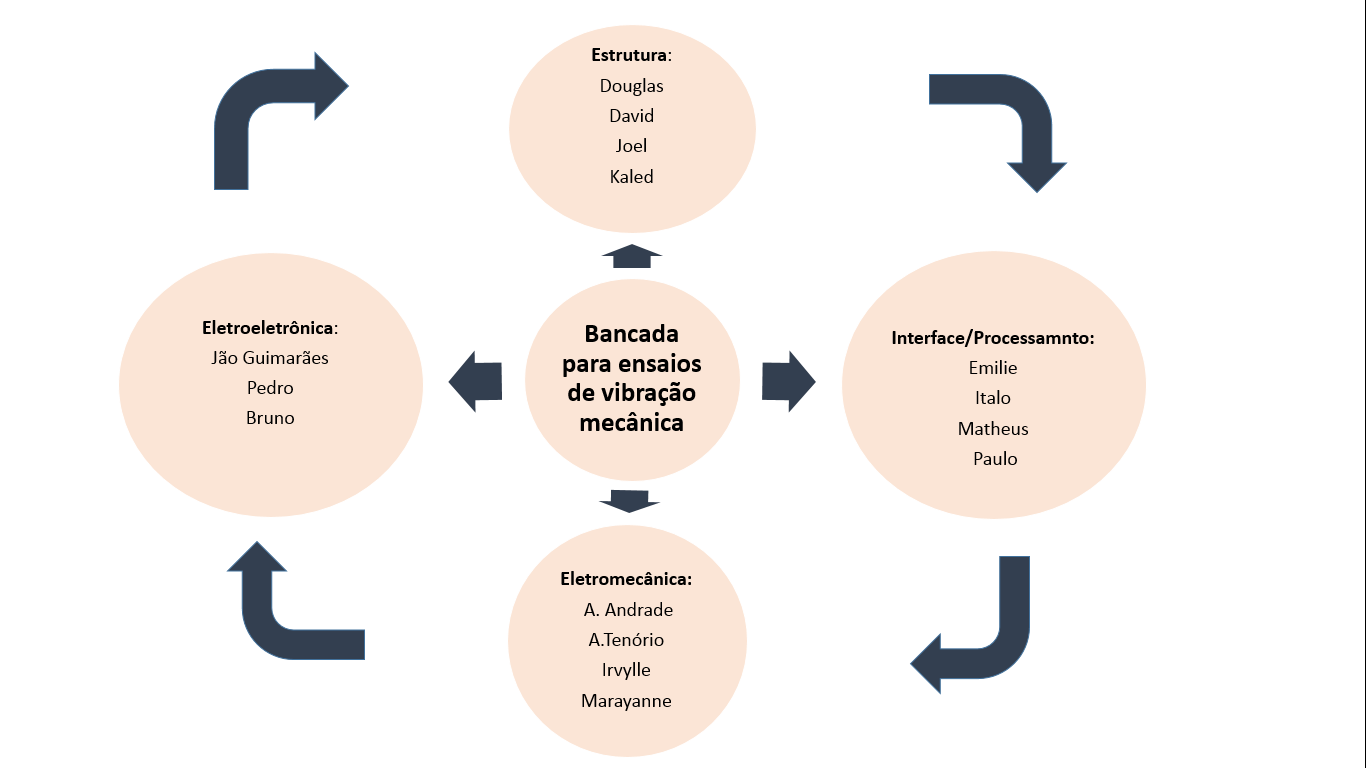
\includegraphics[keepaspectratio=true,scale=0.5]{figuras/organograma.png}
\caption{Organograma da equipe}
\label{organograma}
\end{figure} 

%%%%% CODIGO PRA FIGURA
% \begin{figure}[!ht]
% \centering
% \includegraphics[scale=0.6]{figuras/Organograma.png}
% \caption{Organograma do projeto}
% \label{Organograma}
% \end{figure}
%%%%%%%%%%%%%%%%%%%%%%%%%%%%%%%%%%%%%%%%%%%%%%%%%%%%%

\section*{Avaliação de resultados do projeto}
 Os sistemas de avaliação dos resultados do projeto são feitos a partir de reuniões ocorridas duas vezes na semana (quarta-feira e sexta-feira), nas quais são demonstradas e discutidas as evoluções até então, como também são definidos os próximos passos a serem dados, com base nas determinações já realizadas e nas orientações do que necessita ser feito.

\section*{Frequência da avaliação dos resultados do time}
Os resultados serão apresentados em reuniões com o time e posteriormente com toda a equipe durante as reuniões semanais. Os resultados também são divulgados nas plataformas de comunicação objetivando o esclarecimento de todos da equipe. 


%%%%%%%%%%%%%%%%%%%%%%% FIM PLANO DE GERENCIAMENTO DE RH